%%%%%%%%%%%%%%%%%%%%%%%%%%%%%%%%%%%%%%%%%%%%%%%%%%%%%%%%%%%%%%%%%%% 
%                                                                 %
%                            CHAPTER                              %
%                                                                 %
%%%%%%%%%%%%%%%%%%%%%%%%%%%%%%%%%%%%%%%%%%%%%%%%%%%%%%%%%%%%%%%%%%% 
 
\chapter{Vormgeving van de Robot}
 
%You can say great work has been done about something \citep{Castleman98,Granlund95} or say that \citet{Holmes95} did something really great.




Alvorens aan te vangen met het schrijven van de software en het ontwerpen van de PCB, hebben we onderzocht hoe de robot er zou moeten uitzien om het circuit zo foutloos en snel mogelijk te kunnen afleggen. Een eerste keuze is de plaatsing van het losse wieltje vooraan of achteraan. We bekeken beide opties en besloten dat het losse wieltje vooraan de beste oplossing was aangezien de sensoren zich dan op een grotere afstand bevinden van de stuurwielen. De afstand van sensor tot de stuurwielen zorgt ervoor dat de kleinste fout reeds tot uiting komt en de wielen dus sneller correcties kunnen uitvoeren zodat de fout minimaal blijft. Ook bij de keuze van de geschikte arm zal blijken dat we de afstand tussen de stuurwielen en de sensoren trachten te maximaliseren.

Het oorspronkelijke doel was om onze robot autonoom de circuits te laten rijden met behulp van \'e\'en arm van dertien cm waarop drie sensoren bevestigd zijn zoals te zien in Figuur~\ref{fig:3sensoren}. We hebben dan ook zo snel mogelijk deze arm ontworpen en geprint met de 3D-printer zodat wij onmiddellijk konden beginnen met het schrijven van de software en het afstellen van de motoren en de sensoren met behulp van PID-waarden. Nadat we deze arm aan de rechterkant hadden bevestigd, ging het allemaal vrij snel en hadden we in een mum van tijd een robot die het eerste circuit, het ovale, vloeiend kon afleggen zonder van het parcours te komen. De arm stond 90$^\circ$ gedraaid ten opzichte van de langsas van onze robot waardoor we de afstand tussen de stuurwielen en de sensoren niet maximaliseerden. Nadat we de arm onder een hoek van ongeveer 30$^\circ$ ten opzichte van de langsas van de robot geplaatst hadden, merkten we een grote prestatieverbetering op en konden we de snelheid opdrijven.



\begin{figure}[H]
\centering
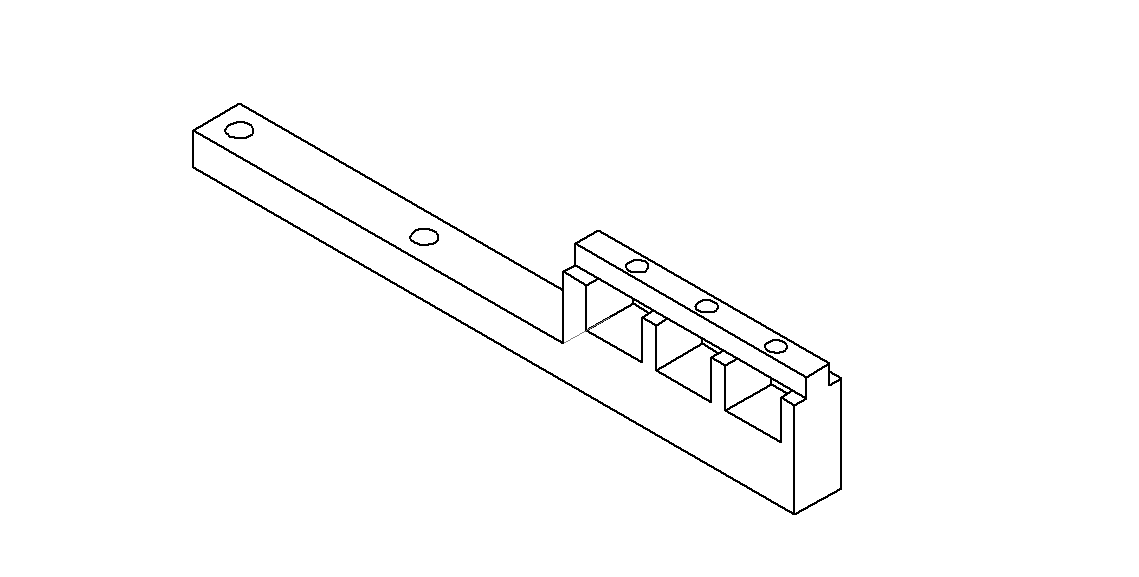
\includegraphics[width=0.75\textwidth]{3sensoren.png}
\caption{Arm voor 3 sensoren. \label{fig:3sensoren}}
\end{figure}


Ons ontwerp was momenteel enkel nog maar in staat om bochten te nemen in 1 richting, namelijk tegenwijzerzin wanneer we de buitenbochten volgden. We begrepen dat ons ontwerp nog niet voldeed om de ingewikkeldere circuits af te leggen waarbij er zowel bochten naar links als naar rechts zouden voorkomen. We hebben vervolgens onderzoek gedaan om de optimale arm te ontwerpen.

De tweede arm die we ontwikkelden, leek sterk op de eerste, maar kon plaats bieden aan 5 sensoren en moest onder eenzelfde hoek geplaatst worden als de bovenstaande arm. We ondervonden echter dat de 2 extra sensoren geen meerwaarde konden bieden aangezien we geen extra foutsituaties konden defini\"eren in onze software omdat de arm niet buiten het circuit mocht komen. 

Ons laatste ontwerp bestaat uit 2 armen, die elkaars spiegelbeeld zijn en waarbij de top van de arm opnieuw een hoek van 30$^\circ$ maakt met de langsas van de robot zoals u kan zien in Figuur \ref{fig:schuinnaarvoor}. U kan dergelijke arm vinden in Figuur \ref{fig:schuinnaarvoor}. Ons doel was dat de armen van de robot zich zo dicht mogelijk bij de buitenlijnen van het circuit bevonden zodat, wanneer de robot afwijkt van de lijn, dit niet zou resulteren in een te grote afwijking van zijn richting. Daarom bezit de arm eerst nog een stuk van 5 cm in de dwarsrichting van de robot zodat de ene arm zich maximaal 2 cm van de buitenlijn bevindt, wanneer de andere zich boven de lijn begeeft. Deze armen bleken voor ons project optimaal en gebruikten we dan ook in ons eindontwerp.

\begin{figure}[H]
\centering
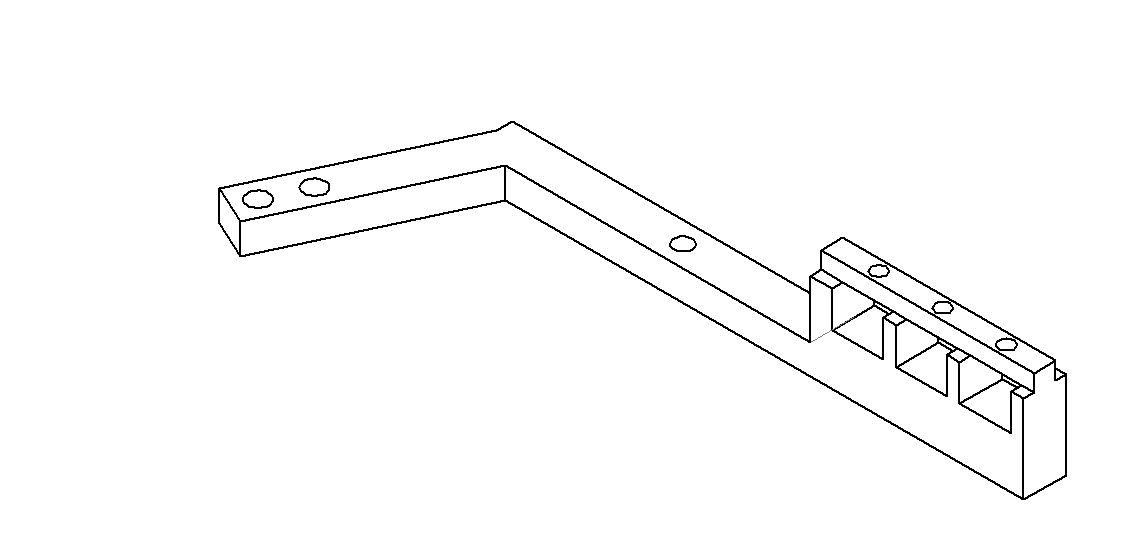
\includegraphics[width=0.75\textwidth]{schuinnaarvoor.png}
\caption{Arm voor sensoren die we gebruiken in ons eindontwerp \label{fig:schuinnaarvoor}}
\end{figure}

We ontwierpen verder ook nog een houder voor de RFID-reader zodat deze zich net voor het losse wieltje zou bevinden. Dit is de plaats waar de robot, en dus ook de RFID-tag, zich met grootste zekerheid boven de lijn bevindt.

Om de snelheid van onze robot te meten, maakten we gebruik van eenzelfde infrarood sensor als de sensoren voor het registreren van de witte lijn. We printten een zwart schijfje met de 3D-printer en maakten een spie van de schijf wit zodat de sensor het wit kon waarnemen en op die manier telkens een rotatie van het wiel kon registreren. De sensor zelf hebben we subtiel met een kleine houder bevestigd onder de robot.

Als laatste gaven we de robot nog vorm met 2 verlengstukjes om een extra printplaat, bedoeld om de bedrading overzichterlijker te maken, te bevestigen en een houder voor de batterij, zodat we deze onderaan konden bevestigen en deze niet meer in de weg zou liggen.

Voor de vormgeving hebben we dus rijkelijk gebruik gemaakt van de 3D-printer waardoor we alles konden positioneren op de exacte plaats waar we het wilden waardoor de robot een afgewerkt geheel werd.



 
%\begin{figure}
%\vspace{2.0in}
%\caption{This is the Caption for Figure 1}
%\end{figure}

 
%\begin{table}[top]
%\begin{center}
%\begin{tabular}{lll}
%Here's       & an          & example  \\
%of           & a           & table    \\
%floated      & with        & the      \\
%\verb+table+ & environment & command.
%\end{tabular}
%\end{center}
%\caption{This is the Caption for Table 1}
%\end{table}
 
%xxx xxxxx xxxxx xxx xxxx xxxx xxxxx xxxxx xxxx xxxxx xxxx xxxxxxxxx
%xxx xxxxx xxxxx xxx xxxx xxxx xxxxx xxxxx xxxx xxxxx xxxx xxxxxxxxx
 